% !TEX root = master.tex

\chapter{Model Order Reduction}
\label{Ch:ROM}
%\pagenumbering{arabic}


In this chapter model order reduction (MOR) of the BGK-model in the Sod shock tube will be introduced for which POD and in particular autoencoders are adopted to obtain a reduced basis (RB).\\
Model order reduction is a technique used for reducing the computational cost when evaluating PDE's \cite{Bernard}\cite{Carlberg}\cite{ohlberger2015reduced}. To achieve this, the solution to the PDE is being approximated by reducing one or more of it's dimensions. The reduction is performed by a mapping onto a low dimensional manifold. In our case the solution to the BGK-model is \(f(x,v,t) \in \mathbb{R}^3\). Now we could reduce i.e. \(v\) to \(n\), with \(o\) beeing the number of elements in \(v\) and \(p\) in \(n\). With \(p << o\) we obtain a reduced order model (ROM) \(q(x,n,t)\) of significantly lower dimension. In particular \(n\) is called the reduced basis or the intrinsic variables. In \cref{Ch:BGK} we saw that the BGK-model is a PDE which through discretization in the spatial dimension \(x\) and the velocity dimension \(v\) holds a system of \(KJ\) ODE's in time in 1D and \(K^3J^3\) ODE's in time in 3D.  By the reduction of \(v\) we arrive at \(nJ\) ODE's in time for 1D and \(nJ^3\) ODE's in time in 3D, though we discuss the 1D case only. This example should illustrate the amount of computations saved by MOR. The mapping from \(f(x,v,t)\) to \(q(x,n,t)\) is implemented through a reduction algorithm, which also performs a remapping back to \(\tilde{f}(x,v,t)\), such that the distance \(||f - \tilde{f}||\) is small.\\
To sum up, the idea that every high dimensional dynamical-state space \(W\), also called solution manifold, which in our case is \(f(x,v,t) \in W\), can be mapped onto a state-space i.e. \(q_n(\mu_i) \in V\)  of lower dimension, is exploited within MOR \cite{ohlberger2015reduced}. Here \(i\) gives the number of variables that are left after the reduction and \(n\) beeing the number of so called intrinsic variables. The state space of lower dimension is called the intrinsic solution manifold \(V\) with \(q_n(\mu_i) \in V\) \cite{Carlberg}.\\
\begin{figure}[H]
	\begin{subfigure}{.45\textwidth}
		\centering
		\tikzstyle{reco} = [rectangle,minimum height=4em,text centered, fill=blue!20,draw=black]
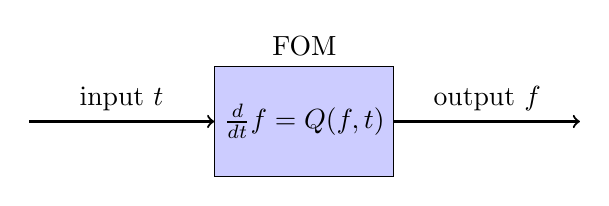
\begin{tikzpicture}[auto]
	\node [reco,label=FOM] (phys) {$\frac{d}{dt}f = Q(f,t)$};
	\draw [<-,thick] (phys)--+ (-3.5,0) node[midway,above] {input \(t\)};
	\draw [->,thick] (phys)--+ (3.5,0) node[midway,above] {output $f$};
\end{tikzpicture}

		\subcaption{Evolving the BGK-model in the Sod shock tube in time is generated through evaluating the FOM in space \(x\), velocity \(v\) and time \(t\), which yields the solution \(f(x,v,t)\). The operator \(Q\) is here the FOM described in \cref{Ch:BGK}.}
	\end{subfigure}\hfill
	\begin{subfigure}{.45\textwidth}
		\centering
		\tikzstyle{reco} = [rectangle,minimum height=4em,text centered, fill=blue!20,draw=black]
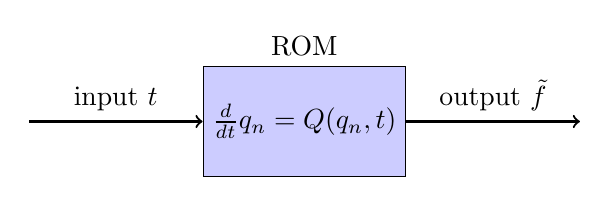
\begin{tikzpicture}[auto]
	\node [reco,label=ROM] (red) {$\frac{d}{dt}q_n = Q(q_n,t)$};
	\draw [<-,thick] (red)--+ (-3.5,0) node[midway,above] {input \(t\)};
	\draw [->,thick] (red)--+ (3.5,0) node[midway,above] {output $\tilde{f}$};
\end{tikzpicture}

		\subcaption{Evolving the ROM of the BGK-model in the Sod shock tube in time through evaluating the ROM at \(n\) and \(\mu_i\), yields an approximation to the FOM solution \(\tilde{f}\). The operator \(Q\) is here either POD or a neural network described in \cref{Ch:DimRedAl}.}
	\end{subfigure}
	\caption{Outline of the correlation between the FOM solution and the approximation obtained from the ROM.}
\end{figure}
MOR is partitioned into two successive phases called the \textit{offline} - and the \textit{online} phase. During the offline phase \textit{snapshots} of a dynamical-system are generated through experiments or simulations of the full order model (FOM). The snapshots \(F = \{f(t1),...,f(t_n)\}\) are created once, each representing one moment in time of the dynamical system. Thus in our case one needs a snapshot database of solutions \(f(x,v,t)\) of the BKG-model in the Sod shock tube. Next a mapping \(Q\) is constructed such that \(\tilde{f} = Q(f)\), for which \(f(t_i) \approx \tilde{f}(t_i)\), reducing the dimensionality of the FOM solution as outlined before. During the online phase the reduced order model is evaluated and the error is estimated by eg. \(||f(t) - \tilde{f}(t)||\). Therefore the online phase may be described as a stage of independence from the full order model.
Following \cite{ohlberger2015reduced} and \cite{Carlberg}, the success when building a ROM through linear reduction methods like the POD \cref{Sec: POD}, depends on a rapidly decaying Kolmogorov N-width. In particular advection dominated problems exhibit a slow decay of the Kolmogorov N-width. Thus yielding a need for non-linear methods like autoencoders described in \cref{Sec:AE}. The Kolmogorov N-width is given by
\begin{equation}
	d_{V}(W):= \sup_{f \in W} \inf_{\tilde{f} \in V} ||f-\tilde{f}||
\end{equation}
and gives the worst best approximation error for elements of \(W\). The convergence behaviour of the Kolmogorov N-width for advection dominated problems, especially when jump conditions are involved as in the Sod shock tube \cref{Ch:BGK}, decays with
\begin{equation}
	d_n(W) \leq \frac{1}{2} n^{-1/2},
\end{equation}
where \(n\) denotes the number of RB or intrinsic variables. Note that hereafter we will solely use the term intrinsic variables\cite{ohlberger2015reduced}. The relevance of this contribution, using non-linear methods for MOR in rarefied gas dynamics, was already implied in the beginning and now takes shape. The BGK-model in the sod shock tube describes an advection problem with jump discontinuities \cref{Ch:BGK}. Thus linear reduction methods should fail. We will see in the following, that this is only partly true, because the advection character as well as the formation of sharp shock fronts heavily depends on the rarefaction of the gas as described in \cref{Ch:BGK}.
\section{Offline Phase}
\subsection{Full order BGK-model}\label{Sec: FOM}
The FOM is the 1D BGK-model in the Sod shock tube for two levels of rarefaction, gratefully provided by Julian K\"ollermeier and the Departement of Mathematics at the RWTH Aachen. The Sod shock tube is discretized in space \(x\) with 100 nodes, in velocity \(v\) with 40 nodes for 25 time steps in time \(t\), as presented in \cref{Tab:Setup} and \cref{Fig:SodProbSetup}. Details about the BGK-model and Sod's shock can be found in \cref{Ch:BGK}.
\begin{table}[htp]
	\centering
	\caption{Problem setup for the BGK model in the Sod shock tube. The diaphragm is positioned at \(x_d=0.5025\). For \(x<x_d\) the gas is present, for \(x\geq x_d\) particles are absent.}
	\begin{tabular*}{15cm}{ @{\extracolsep{\fill}} c c c c @{} }
		\toprule
		Variable   & Number of nodes \(i\)&   Domain extension& Step size (uniform)\\   
		\hline
		\(x\) 		&	200&     [0.0025,0.9975]&	    0.00499\\
		\(v\)       &   40 &  		    [-10,10]&	    0.05128\\
		\(t\)   	&	25 &        	[0,0.12]&	      0.005\\
		\bottomrule
	\end{tabular*} \label{Tab:Setup}
\end{table}
One can be viewed as a slip flow \cite{schaaf} with \(\Kn=0.01\), hereafter referred to as \(\rare\). The dilution up to this level of rarefaction is little though leading to inaccuracies when employing the common Navier Stokes equations. Therefore the NFS-equations (Navier-Stokes-Fourrier) could be used \cite{NumaKUL}. The other is situated in the continuum flow regime with \(\Kn=0.00001\) for which the Navier-Stokes equations can be utilized without hesitation. A detailed description can be found in \cref{Ch:BGK}. Hereafter the continuum flow will be referred to as \(\hy\). Note that both \(\hy\) and \(\rare\) are three dimensional tensors containing \(f(x,v,t)\).\\
The reduction algorithms, introduced in \cref{Ch:DimRedAl}, require a distinct reshaping of the input data before they can be used. The preprocessed matrix for the FCNN, \(\mae\), is shown in \cref{Eq:AE_matrix}. Each row of \(\mae\) contains a sample shown to the FCNN. In turn we aquire \(x_it_i=5000\) samples. The preprocessed matrix for the CNN, \(\mconv\), is shown in \cref{Eq:CNN_matrix}. We obtain \(v_i=40\) samples, each containing a matrix \(\pi_{CNN}^{x_i\times t_i}\) holding the information about \(f(x,t)\) for a fixed point in \(v\). POD uses the \(\mae\) matrix or its transposition.\\
\begin{minipage}{.55\linewidth}
	\begin{equation}
	\mae = \begin{bmatrix}
	f(v_1,t_1,x_1)&\cdots &f(v_n,t_1,x_1) \\
	f(v_1,t_1,x_2)&\cdots &f(v_n,t_1,x_2) \\
	\vdots& \vdots & \vdots\\
	f(v_1,t_1,x_n)&\cdots &f(v_n,t_1,x_n)\\
	f(v_1,t_2,x_1)&\cdots &f(v_n,t_2,x_1)\\
	\vdots & \vdots & \vdots\\
	f(v_1,t_n,x_n)&\cdots &f(v_n,t_n,x_n)
	\end{bmatrix}
	\label{Eq:AE_matrix}
	\end{equation}
\end{minipage}%
\begin{minipage}{.45\linewidth}
	\begin{equation}
	\mconv= \begin{bmatrix}
	n_{Filters},&f(v_1,\textbf{t},\textbf{x})\\
	n_{Filters},&f(v_2,\textbf{t},\textbf{x})\\
	\vdots&\vdots\\
	n_{Filters},&f(v_n,\textbf{t},\textbf{x})
	\end{bmatrix}
	\label{Eq:CNN_matrix}
	\end{equation}
\end{minipage}\\\\
In the following a distinction between \(\mconv\) and \(\mae\) is omitted, when referring to the preprocessed matrices. However a distinction between the levels of rarefaction, namely \(\hy\) and \(\rare\), will be utilized as \(\mhy\) for the former and \(\mrare\) for the latter. This designation is mainly used in \cref{Ch:ApB} and \cref{Ch:ApA}.
\subsection{Contructing the mapping}
With the FOM solution at hand it is possible to construct a mapping \(Q\) such that \(Q(f)\approx \tilde{f}\). For \(Q\), POD and two autoencoders, based on a fully connected neural network (FCNN) and a convolutional neural network (CNN), are employed, see \cref{Ch:DimRedAl}. The architecture, selection of hyperparameters and training for the FCNN and the CNN is discussed in \cref{Sec:AppendixA}. Hence the existence of fully trained and tuned FCNN and CNN is given from now on. Since this thesis mainly focuses on methods from machine learning, POD serves as a comparative measure. To continue, the intrinsic variables obtained from POD, the FCNN and the CNN, will be referred as \(\idhy\) and \(\idrare\). The former describes the intrinsic variables when reducing \(\hy\) and the latter when reducing \(\rare\).\\
In order to choose the number \(n\) of intrinsic variables (sizes of \(\idhy\) and \(\idrare\)) we will utilized POD as a reference framework. Therefore the singular values \(\sigma\), as well as, the cumulative energy (cusum-e)\\
\noindent \begin{minipage}{.3\linewidth}
	\begin{equation}
	\textrm{cusum-e} = \frac{\textrm{cusum}}{\sum_i \sigma_i}
	\end{equation}
\end{minipage}%
\begin{minipage}{.7\linewidth}
	\begin{equation}
			\textrm{with} \qquad\qquad(\textrm{cusum})_i =(\text{cusum})_{i-1} + \sigma_{i}
	\end{equation}
\end{minipage}\\\\
over the singular values, are employed. A comparison for both levels of rarefaction is provided in \cref{Fig:CUSUM-e}. With only \(n=4\) intrinsic variables, \\
From a physical point of view the number of intrinsic variables for \(\hy\) should be in total not more than three, as a slip-flow can be described in terms of three macroscopic quantities like density \(\rho\), macroscopic velocity \(u\) and total energy \(E_{tot}\)\cite{BGK}\cite{Bernard}. Therefore \(n=3\) is employed for \(\idhy\). When considering \(\rare\) the picture becomes a little blurrier.  \\

As announced earlier, does the decay of the Kolmogorov n-width depend on the formation of sharp shock fronts, which in turn depends on the level of rarefaction in the Sod shock tube. Rarefied gases exhibit a diffusion dominated behavior whereas with increasing compression, the advection behavior becomes gradually dominant, see \cref{Ch:BGK}. 
\begin{figure}[!htbp]
	\begin{subfigure}{.45\textwidth}
		% This file was created by tikzplotlib v0.9.6.
\begin{tikzpicture}

\begin{groupplot}[group style={group size=2 by 1, horizontal sep=1cm, vertical sep=2cm}]
\nextgroupplot[
log basis y={10},
tick align=outside,
tick pos=left,
x grid style={white!69.0196078431373!black},
xlabel={\(k\)},
xmin=-1.95, xmax=40.95,
xtick style={color=black},
y grid style={white!69.0196078431373!black},
ylabel={\(\sigma\)},
ymin=5.00425450746683e-16, ymax=233.601752047754,
ymode=log,
ytick style={color=black},
width=.6\textwidth,
height=.7\textwidth,
ytick={1e1,1e-3,1e-11,1e-15},
width=.55\textwidth,
height=.7\textwidth,
y label style={yshift=-2.5em},
grid=both
]
\addplot [semithick, red, mark=o, mark size=2, mark options={solid}]
table {%
0 36.7564464709921
1 6.45572768708393
2 2.70096946740729
3 0.706165973805752
4 0.280354602766687
5 0.102537716843524
6 0.0440340620127454
7 0.0218638471526527
8 0.00685281169963933
9 0.00206424289417759
10 0.00100028680918087
11 0.0002164070851145
12 0.000192016045990026
13 2.76177875569651e-05
14 1.65500681978358e-05
15 2.40203186862594e-06
16 1.13376480492873e-06
17 1.54303137841961e-07
18 6.12006889847331e-08
19 7.054966207969e-09
20 2.62311702138279e-09
21 2.48217436010154e-10
22 8.81706226450051e-11
23 6.88254148471367e-12
24 2.27942669067321e-12
25 1.42331417671071e-13
26 4.36913792303503e-14
27 1.63220898105638e-14
28 3.18040162440537e-15
29 3.18040162440537e-15
30 3.18040162440537e-15
31 3.18040162440537e-15
32 3.18040162440537e-15
33 3.18040162440537e-15
34 3.18040162440537e-15
35 3.18040162440537e-15
36 3.18040162440537e-15
37 3.18040162440537e-15
38 3.18040162440537e-15
39 3.18040162440537e-15
};

\nextgroupplot[
tick align=outside,
tick pos=left,
x grid style={white!69.0196078431373!black},
xlabel={\(k\)},
xmin=-1.95, xmax=40.95,
xtick style={color=black},
y grid style={white!69.0196078431373!black},
ylabel={cum-sum},
ymin=0.769785900167041, ymax=1.01096257618252,
ytick style={color=black},
ytick={1,.8},
width=.55\textwidth,
height=.7\textwidth,
y label style={yshift=-2em},
grid=both
]
\addplot [semithick, red, mark=o, mark size=2, mark options={solid}]
table {%
0 0.780748476349562
1 0.917875430648483
2 0.975247075592702
3 0.990246839199716
4 0.996201887904449
5 0.998379904929493
6 0.999315238187322
7 0.999779651018009
8 0.999925212485639
9 0.999969059338346
10 0.999990306561001
11 0.999994903292138
12 0.99999898193003
13 0.99999956856306
14 0.999999920105218
15 0.99999997112709
16 0.999999995209537
17 0.99999999848711
18 0.999999999787082
19 0.999999999936937
20 0.999999999992655
21 0.999999999997927
22 0.9999999999998
23 0.999999999999946
24 0.999999999999995
25 0.999999999999998
26 0.999999999999999
27 0.999999999999999
28 0.999999999999999
29 0.999999999999999
30 0.999999999999999
31 0.999999999999999
32 0.999999999999999
33 0.999999999999999
34 0.999999999999999
35 0.999999999999999
36 0.999999999999999
37 0.999999999999999
38 0.999999999999999
39 0.999999999999999
};
\end{groupplot}

\end{tikzpicture}

		\subcaption{Sigular values \(\sigma\) over \(k\) number of singular values (left) and cumulative energy, here labeled as \glqq cusum-e\grqq{} over \(k\) (right) for \(\hy\). A black cross marker corresponds to over 99\% cumulative energy.}
		\label{Fig:CumSum_Rare}
	\end{subfigure}\hfill
	\begin{subfigure}{.45\textwidth}
		% This file was created by tikzplotlib v0.9.6.
\begin{tikzpicture}

\begin{groupplot}[group style={group size=2 by 1, horizontal sep=1cm, vertical sep=2cm}]
\nextgroupplot[
log basis y={10},
tick align=outside,
tick pos=left,
x grid style={white!69.0196078431373!black},
xlabel={\(k\)},
xmin=-0.95, xmax=41.95,
xtick style={color=black},
y grid style={white!69.0196078431373!black},
ylabel={\(\sigma\)},
ymin=5.00425450746683e-16, ymax=233.601752047754,
ymode=log,
ytick style={color=black},
width=.6\textwidth,
height=.7\textwidth,
ytick={1e1,1e-3,1e-11,1e-15},
width=.55\textwidth,
height=.7\textwidth,
y label style={yshift=-2.5em},
grid=both
]
\addplot [semithick, red, mark=o, mark size=2, mark options={solid}]
table {%
1 36.7564464709921
2 6.45572768708393
3 2.70096946740729
4 0.706165973805752
5 0.280354602766687
6 0.102537716843524
7 0.0440340620127454
8 0.0218638471526527
9 0.00685281169963933
10 0.00206424289417759
11 0.00100028680918087
12 0.0002164070851145
13 0.000192016045990026
14 2.76177875569651e-05
15 1.65500681978358e-05
16 2.40203186862594e-06
17 1.13376480492873e-06
18 1.54303137841961e-07
19 6.12006889847331e-08
20 7.054966207969e-09
21 2.62311702138279e-09
22 2.48217436010154e-10
23 8.81706226450051e-11
24 6.88254148471367e-12
25 2.27942669067321e-12
26 1.42331417671071e-13
27 4.36913792303503e-14
28 1.63220898105638e-14
29 3.18040162440537e-15
30 3.18040162440537e-15
31 3.18040162440537e-15
32 3.18040162440537e-15
33 3.18040162440537e-15
34 3.18040162440537e-15
35 3.18040162440537e-15
36 3.18040162440537e-15
37 3.18040162440537e-15
38 3.18040162440537e-15
39 3.18040162440537e-15
40 3.18040162440537e-15
};

\nextgroupplot[
tick align=outside,
tick pos=left,
x grid style={white!69.0196078431373!black},
xlabel={\(k\)},
xmin=-0.95, xmax=41.95,
xtick style={color=black},
y grid style={white!69.0196078431373!black},
ylabel={cusum-e},
ymin=0.769785900167041, ymax=1.01096257618252,
ytick style={color=black},
ytick={1,.8},
width=.55\textwidth,
height=.7\textwidth,
y label style={yshift=-2em},
grid=both
]
\addplot [semithick, red, mark=o, mark size=2, mark options={solid}]
table {%
1 0.780748476349562
2 0.917875430648483
3 0.975247075592702
4 0.990246839199716
5 0.996201887904449
6 0.998379904929493
7 0.999315238187322
8 0.999779651018009
9 0.999925212485639
10 0.999969059338346
11 0.999990306561001
12 0.999994903292138
13 0.99999898193003
14 0.99999956856306
15 0.999999920105218
16 0.99999997112709
17 0.999999995209537
18 0.99999999848711
19 0.999999999787082
20 0.999999999936937
21 0.999999999992655
22 0.999999999997927
23 0.9999999999998
24 0.999999999999946
25 0.999999999999995
26 0.999999999999998
27 0.999999999999999
28 0.999999999999999
29 0.999999999999999
30 0.999999999999999
31 0.999999999999999
32 0.999999999999999
33 0.999999999999999
34 0.999999999999999
35 0.999999999999999
36 0.999999999999999
37 0.999999999999999
38 0.999999999999999
39 0.999999999999999
40 0.999999999999999
};
\addplot [thick, , mark=x,black, mark size=2, mark options={solid}]
table{%
4 0
4 0.990246839199716
4 1.3
};
\end{groupplot}

\end{tikzpicture}

		\subcaption{Sigular values \(\sigma\) over \(k\) number of singular values (left) and cumulative energy, here labeled as \glqq cusum-e\grqq{} over \(k\) (right) for \(\rare\).  A black cross marker corresponds to over 99\% cumulative energy.}
		\label{Fig:CumSum_Hydro}
	\end{subfigure}
	\caption{Comparison of singular variables \(\sigma\) and cumulative energy for \(hy\) and \(\rare\). The decay of the singular values can be used to estimate the decay of the Kolmogorov n-width.}
	\label{Fig:CUSUM-e}
\end{figure}
\begin{table}[!htbp]
	\centering
	\caption{}
	\begin{tabular*}{16.5cm}{ @{\extracolsep{\fill}} c c c c c c c c c c c @{} }
		\toprule
		Intrinsic variables&  2 & 3 &  4  &  5  & 6  & 7  & 8  & 9  & 10 \\   
		\hline
		\(\L2\)-Error for \(\rare\)& 0.0750 & 0.0205 &0.0081& 0.0030& 0.0013& 0.0006& 0.0002& 6.2\(e^{-5}\)& 2.7\(e^{-5}\) \\
		\(\L2\)-Error for \(\hy\)&0.0853 & 0.0327 & 0.0153 & 0.0087 & 0.0046 & 0.0021 & 0.0014 & 0.0005 & 0.0003\\
		\bottomrule
	\end{tabular*} \label{Tab:NumIntVar}
\end{table}

\subsection{Online Phase}
loremipsu
\subsection{Reduced Order Model}\label{Reduced Order Model}
The compression of the input data $y_0$ yields a code $C \in \mathbb{R}^{ix5000}$, composed  of the instrinsic variables \(c_i\). The index \(i\) corresponds to the i-th intrinsic variable whereas their number is given by the input data. Each of them describes the transport of a discontinuity as seen in \cref{Fig:Code_Fully}. Hence the expolitability of the code in terms of constructing a ROM is not provided. On that account the method of characteristics \cite{Dret2016} provides a means to bypass this shortage. It is necessary for $c_i(x,t)$ to satisfy the conservative condition \cref{Eq. Mass_Const} and the transport equation \cref{Eq. Transport}.\\
\noindent\begin{minipage}{.5\linewidth}
	\begin{equation}
	\frac{d}{dt}\int c_i\ dx = \frac{d}{dt}f_i = const. \label{Eq. Mass_Const}
	\end{equation}
\end{minipage}%
\begin{minipage}{.5\linewidth}
	\begin{equation}
	\frac{\partial}{\partial t}c_i + \frac{\partial}{\partial x}f_i = 0 \label{Eq. Transport}
	\end{equation}
\end{minipage}
The characteristics $u_i$ describe the constant transport velocities for each variable $c_i$ calculated using \cref{Eq. Characteristics}. Subsequently enabling the usage of a simple plynomial interpoaltion of any degree. Furthermore a linear mapping \(A_ix_i=c_i\) can be applied for the reconstruction of interpolated code variables \(\hat{c}_i\). \Cref{Fig. Flowchart} depicts this approach in detail.\\
Questions concering the capacity of this ROM, e.g. how many samples \(\hat{n}_t\) are needed to reconstruct \(n_t\) timestamps, are analysed in \cref{Results}.
\begin{equation}
	u_i = \frac{f_i(c^-_i) - f_i(c^+_i)}{c^-_i - c^+_i}
	\label{Eq. Characteristics}
\end{equation}
\begin{figure}
	\centering
	\usetikzlibrary{matrix}
\usetikzlibrary{shapes,snakes}
	\tikzstyle{rec} = [rectangle, rounded corners, minimum width=1cm, minimum height=1cm,text centered, draw=black]
	\tikzstyle{circ} = [circle,minimum size =1.5cm,text centered, draw=black]
	\tikzstyle{arrow} = [thick,->,>=stealth]
		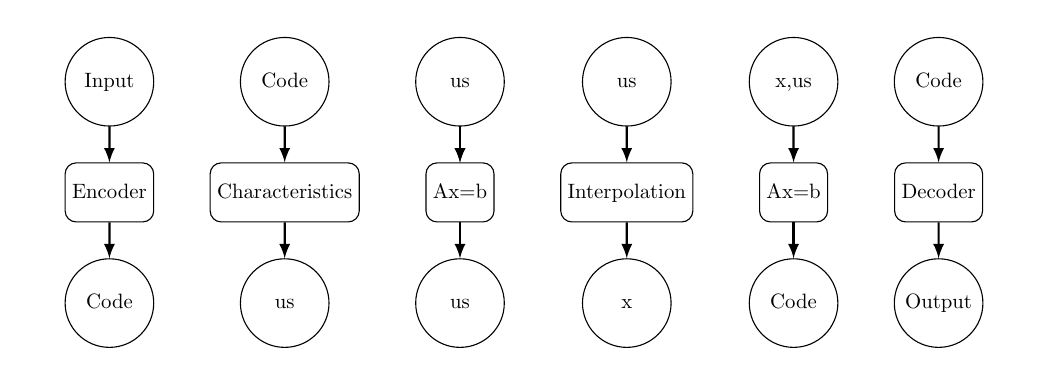
\begin{tikzpicture}[>=latex,text height=1.5ex,text depth=0.25ex,scale=.5,every node/.style={scale=0.75}]
		\matrix[matrix of nodes,column sep= 1em,row sep= 3ex]{
			&
			\node[circ] (1) {Input};&
			&
			\node[circ] (4) {Code};&
			&
			\node[circ] (7) {us};&
			&
			\node[circ] (10) {us};&
			&
			\node[circ] (13) {x,us};&
			&
			\node[circ] (16) {Code};&
			\\
			&
			\node[rec] (2) {Encoder};&
			&
			\node[rec] (5) {Characteristics};&
			&
			\node[rec] (8) {Ax=b};&
			&
			\node[rec] (11) {Interpolation};&
			&
			\node[rec] (14) {Ax=b};&
			&
			\node[rec] (17) {Decoder};&
			\\
			&
			\node[circ] (3) {Code};&
			&
			\node[circ] (6) {us};&
			&
			\node[circ] (9) {us};&
			&
			\node[circ] (12) {x};&
			&
			\node[circ] (15) {Code};&
			&
			\node[circ] (18) {Output};&
			\\
		};
	\path[->]
		(1) edge[thick] (2)
		(2) edge[thick] (3)
		(4) edge[thick] (5)
		(5) edge[thick] (6)
		(7) edge[thick] (8)
		(7) edge[thick] (8)
		(8) edge[thick] (9)
		(10) edge[thick] (11)
		(11) edge[thick] (12)
		(13) edge[thick] (14)
		(14) edge[thick] (15)
		(16) edge[thick] (17)
		(17) edge[thick] (18);
\end{tikzpicture}
	\caption{This figure shows the steps for obtaining a reduced oder model (ROM). Decoder and Encoder need to be used after training. In step one $y_0$ is the original input data, $C$ is the Code. In step two $c_i$ is the i-th intrinsic variable and $u_i$ the correspnding characteristic. The eigenvalue problem in step 3 outputs $x_i$ the eigenvector of A, a diagonal matrix composed of $u_i$ and b is the corresponing i-th intrinsic variable $c_i$. In step 4 $\hat{u}_i$ is the interpolated vector to $u_i$. Step 5 solves the linear equation for the diagonal matrix A composed of $\hat{u}_i$ times the eigenvector $x_i$ of the eigenvalueproblem in step 3. The output is $\hat{c}_i$ the i-th intrinsic variable corresponding to $\hat{u}_i$ the i-th interpolated characteristic.}
	\label{Fig. Flowchart}
\end{figure}